\subsection{Avatar cropping}

While the previous section described how the user avatar can be set, this one explains how the cropping of images that are not in the correct aspect ratio is being done. All avatars have to be in a square aspect ratio. However, not all users have to skills to provide an image that meets these requirements. So we decided to crop uploaded images into the appropriate format as they are being uploaded.

What we do is taking the shortest of the two rectangle sides and cut a partial from the center of the longer one of the two sides, which has the same length as the shortest side. To make it more visual, what that means, figure \ref{fig:cropping-avatar} shows an example. The red area is the part that will be cropped.

\begin{figure}[!h]
  \centering
  \fbox{
    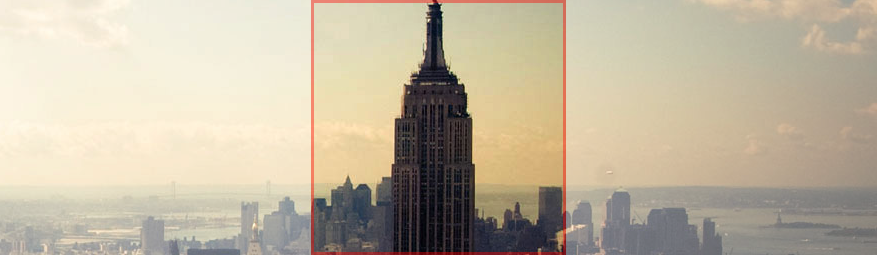
\includegraphics[width=0.97\textwidth]{images/cropped-avatar.png}
  }
  \caption{Cropping avatar}
  \label{fig:cropping-avatar}
\end{figure}

The cropped image then is being scaled to the needed width and height, currently 50 x 50 pixels. The algorithm for cropping that has been developed, is shown in the following code snippet.

\begin{lstlisting}[caption=Cropping an image to a square aspect ratio]
public function crop($thumbWidth, $thumbHeight){
    //getting the image dimensions
    list($width, $height) = getimagesize($this->file->getFullPath());
    
    //saving the image into memory (for manipulation with GD Library)
    $myImage = imagecreatefromjpeg($this->file->getFullPath());

    // setting the crop size
    if($width < $height) {
      $twidth = $width;
      $theight = $width;
      $x = 0;
      $y = $height / 2. - $width / 2.;
    } else {
      $twidth = $height;
      $theight = $height;
      $x = $width / 2. - $height / 2.;
      $y = 0;
    }

    // creating the thumbnail
    $thumb = imagecreatetruecolor($thumbWidth, $thumbHeight);
    imagecopyresampled($thumb, $myImage, 0, 0, $x, $y, $thumbWidth, $thumbHeight, $twidth, $theight);

    imagejpeg($thumb, $this->file->getFullPath());

    imagedestroy($thumb);
    imagedestroy($myImage);

    return $this->file;
  }
\end{lstlisting}
